\documentclass[a4paper,11pt,oneside]{book}
\usepackage{tikz,pgfplots}
\usepackage{hyperref}

\begin{document}

\subsection*{Figure 2.1}
See \href{https://tex.stackexchange.com/questions/299537/gravitational-electric-field-with-tikzpicture}{Here}

\subsection*{Figure 2.2}
See \href{https://tex.stackexchange.com/questions/392942/how-to-draw-force-lines-onto-an-equipotential-contour-plot-using-tikz?rq=1}{here}
\subsection*{Figure 2.3}
\begin{tikzpicture}[scale=0.95]
\begin{axis}[
    axis lines=middle,
    xmin=-4, xmax=4,
    ymin=-2, ymax=1,
    xlabel = $x$,
    ylabel = $V$,
]
%Below the red is defined
\addplot [
    domain=-10:10, 
    samples=100, 
    color=red,
    style={ultra thick}
]
{-2^(-x^2)};
\addlegendentry{$V(x)$}

\end{axis}
\end{tikzpicture}
\subsection*{Figure 2.4}
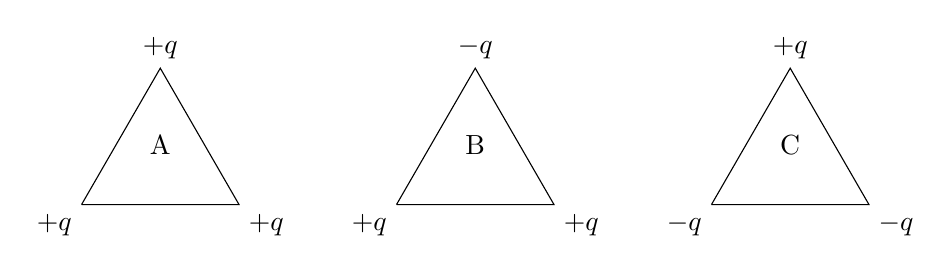
\begin{tikzpicture}
\draw (0,0) -- (2,0) -- (1,1.732) -- (0,0);
\node[below left] at (0,0) {$+q$};
\node[below right] at (2,0) {$+q$};
\node[above] at (1,1.732) {$+q$};
\node[below] at (1,1) {A};

\draw (4,0) -- (6,0) -- (5,1.732) -- (4,0);
\node[below left] at (4,0) {$+q$};
\node[below right] at (6,0) {$+q$};
\node[above] at (5,1.732) {$-q$};
\node[below] at (5,1) {B};

\draw (8,0) -- (10,0) -- (9,1.732) -- (8,0);
\node[below left] at (8,0) {$-q$};
\node[below right] at (10,0) {$-q$};
\node[above] at (9,1.732) {$+q$};
\node[below] at (9,1) {C};

\end{tikzpicture}

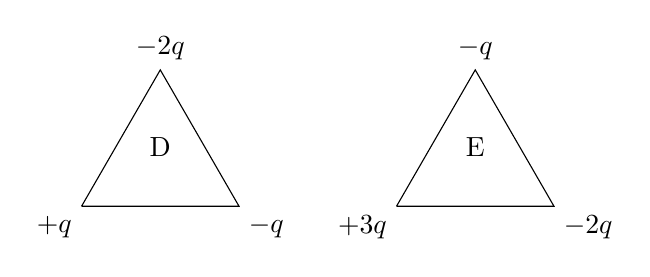
\begin{tikzpicture}
\draw (0,0) -- (2,0) -- (1,1.732) -- (0,0);
\node[below left] at (0,0) {$+q$};
\node[below right] at (2,0) {$-q$};
\node[above] at (1,1.732) {$-2q$};
\node[below] at (1,1) {D};

\draw (4,0) -- (6,0) -- (5,1.732) -- (4,0);
\node[below left] at (4,0) {$+3q$};
\node[below right] at (6,0) {$-2q$};
\node[above] at (5,1.732) {$-q$};
\node[below] at (5,1) {E};

\end{tikzpicture}
\subsection*{Figure 2.5}
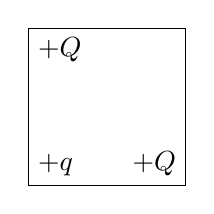
\begin{tikzpicture}
\draw (0,0) -- (0,2) -- (2,2) -- (2,0) -- (0,0);
\node[above right] at (0,0) {$+q$};
\node[below right] at (0,2) {$+Q$};
\node[above left] at (2,0) {$+Q$};
\end{tikzpicture}
\subsection*{Figure 2.6}
\begin{tikzpicture}
\begin{axis}[
    axis lines=middle,
    xmin=0, xmax=2,
    ymin=0, ymax=2,
    xtick=1, ytick=1,
    xlabel = $x$,
    ylabel = $y$,
]
\addplot [only marks] table {
1   0
0   1
};

\addplot [domain=-10:10, samples=2, dashed] {1-x};
\end{axis}
\end{tikzpicture}
\subsection*{Figure 2.7}
\begin{center}
  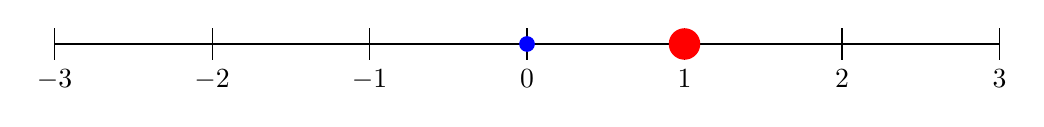
\begin{tikzpicture}[scale=2]
    \draw (-3,0) -- (3,0);
    \foreach \i in {-3,-2,...,3} numbers on line
      \draw (\i,0.1) -- + (0,-0.2) node[below] {$\i$};
    \fill[blue] (0,0) circle (0.5 mm);
    \fill[red]  (1,0) circle (1 mm);
  \end{tikzpicture}   
\end{center}

\subsection*{Figure 2.8}
\begin{tikzpicture}
\begin{axis}[
    axis lines=middle,
    xmin=-20, xmax=20,
    ymin=-20, ymax=20,
    xlabel = $x$,
    ylabel = $V$,
]
%Below the red is defined
\addplot [
    domain=-20:20, 
    samples=100, 
    color=red,
    style={ultra thick}
]
{-1/(x^2)};
\addlegendentry{$V_{-q}$}

%Here the blue is defined
\addplot [
    domain=-20:20, 
    samples=100, 
    color=blue,
    style={ultra thick},
]
{17*x/((6-x)^2)};
\addlegendentry{$V_{17q}$}

\end{axis}
\end{tikzpicture}
\subsection*{Figure 2.9}
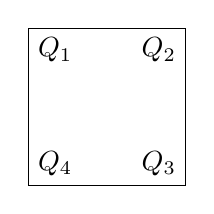
\begin{tikzpicture}
\draw (0,0) -- (0,2) -- (2,2) -- (2,0) -- (0,0);
\node[above right] at (0,0) {$Q_4$};
\node[below right] at (0,2) {$Q_1$};
\node[below left] at (2,2) {$Q_2$};
\node[above left] at (2,0) {$Q_3$};
\end{tikzpicture}
\subsection*{Figure 2.10}
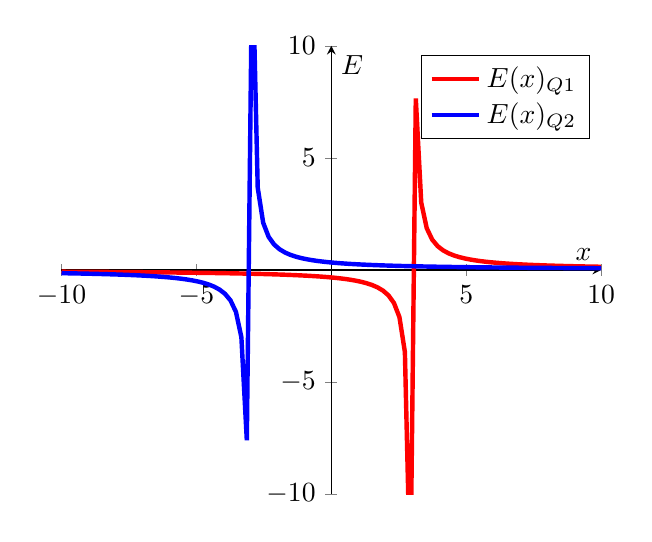
\begin{tikzpicture}
\begin{axis}[
    axis lines=middle,
    xmin=-10, xmax=10,
    ymin=-10, ymax=10,
    xlabel = $x$,
    ylabel = $E$,
]
%Below the red is defined
\addplot [
    domain=-10:10, 
    samples=100, 
    color=red,
    style={ultra thick}
]
{1/(x-3)};
\addlegendentry{$E(x)_{Q1}$}

%Here the blue is defined
\addplot [
    domain=-10:10, 
    samples=100, 
    color=blue,
    style={ultra thick},
]
{1/(x+3)};
\addlegendentry{$E(x)_{Q2}$}

\end{axis}
\end{tikzpicture}

\subsection*{Figure 2.11}
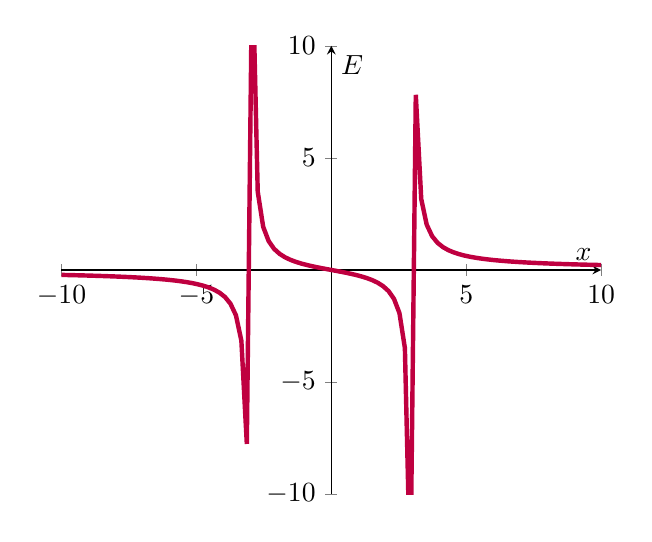
\begin{tikzpicture}
\begin{axis}[
    axis lines=middle,
    xmin=-10, xmax=10,
    ymin=-10, ymax=10,
    xlabel = $x$,
    ylabel = $E$,
]

%Here the purple is defined
\addplot [
    domain=-10:10, 
    samples=100, 
    color=purple,
    style={ultra thick},
]
{(1/(x+3))+(1/(x-3))};

\end{axis}
\end{tikzpicture}
\end{document}